В ближайшее время вам предстоит сдать экзамен по истории искусств, но вы
занимались информатикой существенно больше, чем искусством! Поэтому нужно
написать программу, которая сдаст экзамен за вас.

В экзаменационном задании используется несколько картин. Каждая картина
относится к одному из четырех стилей, пронумерованных 1, 2, 3 и 4.

Стиль 1: неопластицизм. Например:

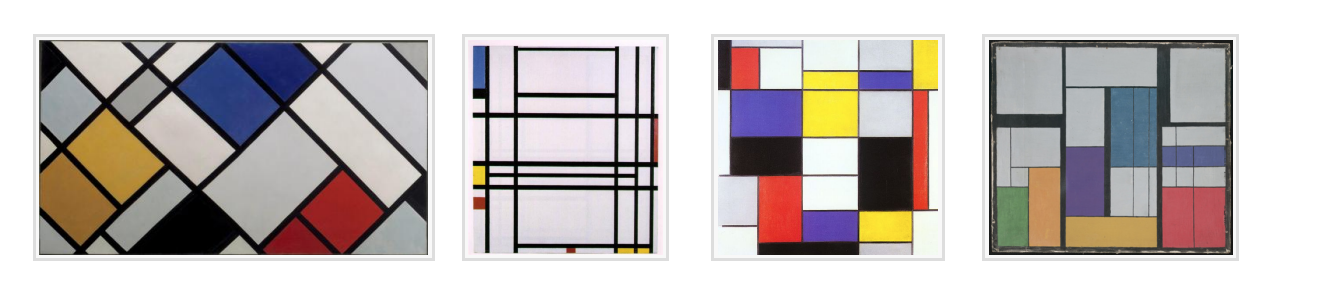
\includegraphics[scale=0.8]{artclass1.png}

Стиль 2: импрессионистский пейзаж. Например:

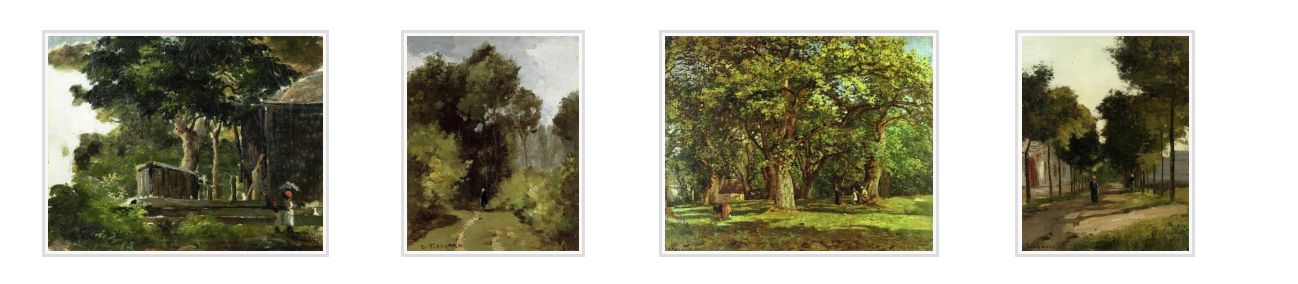
\includegraphics[scale=0.8]{artclass2.png}

Стиль 3: экспрессионистская живопись действия. Например:

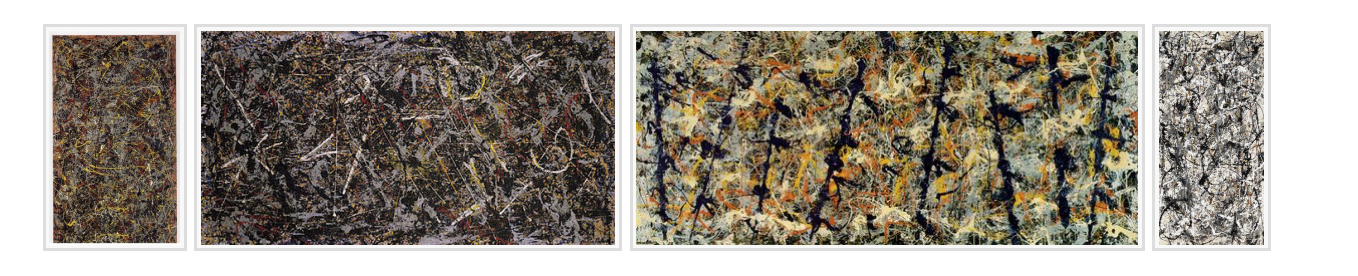
\includegraphics[scale=0.8]{artclass3.png}

Стиль 4: живопись цветового поля. Например:

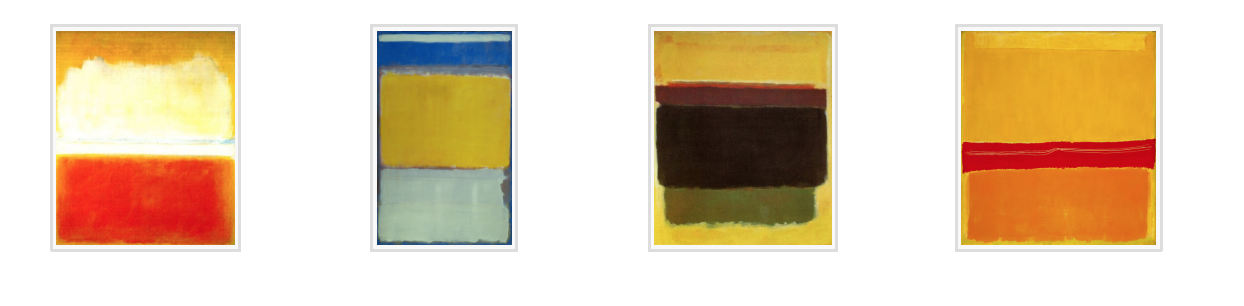
\includegraphics[scale=0.8]{artclass4.png}

Ваша задача состоит в том, чтобы по цифровому образу картины определить, к
какому из стилей она принадлежит.

Научный комитет международной олимпиады по информатике собрал много картин
каждого стиля. Девять случайно выбранных картин каждого стиля включены в
материалы этой задачи, которые вы можете скачать в секции материалы задачи. Каждая из них содержится в виде jpeg-файла который можно посмотреть и в виде текстововго файла который был бы отдан на ввод вашей программе. Вы можете изучить их и использовать для локального тестирования. Остальные картины будут даны вашей
программе во время тестирования в системе.

Цифровой образ картины представляет собой таблицу из $H \times W$ пикселей. Строки
таблицы пронумерованы от $0$ до $H ­- 1$ сверху вниз, а столбцы пронумерованы от
$0$ до $W -­ 1$ слева направо.

Таблица описывается тремя двумерными массивами $R$, $G$ и $B$, которые для
каждого пикселя цифрового образа задают интенсивность красного, зеленого и
синего цветов, соответственно. Интенсивность находится в пределах от $0$ (нет
красного, зеленого или синего цвета) до $255$ (максимальная интенсивность
красного, зеленого или синего цвета).

Ваше решение должно реализовывать нижеописанную функцию \t{style()} на С/C++:

\t{int style(int H, int W, int R[500][500], int G[500][500], int B[500][500]);}


Эта функция должна определять стиль картины.

Параметры:
\begin{itemize}
\item $H$: количество строк пикселей в цифровом образе.
\item $W$: количество столбцов пикселей в цифровом образе.
\item $R$: двумерный массив размера $H \times W$, задающий интенсивность красного цвета в каждом пикселе цифрового образа.
\item $G$: двумерный массив размера $H \times W$, задающий интенсивность зеленого цвета в каждом пикселе цифрового образа.
\item $B$: двумерный массив размера $H \times W$, задающий интенсивность синего цвета в каждом пикселе цифрового образа.
\item \textit{Возвращаемое значение}: стиль картины, который должен быть равен $1$, $2$, $3$ или $4$, как описано выше.
\end{itemize}

Элемент каждого из массивов $R[i][j]$, $G[i][j]$ и $B[i][j]$ соответствует
пикселю в строке $i$, в столбце $j$ и является целым числом от $0$ до $255$
включительно.